\documentclass[12pt]{article}
%\usepackage{geometry}                % See geometry.pdf to learn the layout options. There are lots.
%\geometry{letterpaper}                   % ... or a4paper or a5paper or ... 
%\geometry{landscape}                % Activate for for rotated page geometry
\usepackage[parfill]{parskip}    % Activate to begin paragraphs with an empty line rather than an indent
\usepackage{daves,fancyhdr,natbib,graphicx,dcolumn,amsmath,lastpage,url}
\usepackage{amsmath,amssymb,epstopdf,longtable}
\usepackage{paralist}  % need to properly formulate standard answer blocks
\usepackage[final]{pdfpages}
\usepackage{multicol}
\usepackage{booktabs}
\DeclareGraphicsRule{.tif}{png}{.png}{`convert #1 `dirname #1`/`basename #1 .tif`.png}
\pagestyle{fancy}
\lhead{CE 3372 Water Systems Design; Exam 3}
\rhead{}%Name:\_\_\_\_\_\_\_\_\_\_\_\_\_\_\_\_\_\_\_\_\_\_\_\_\_\_\_\_\_\_\_\_\_\_}
\lfoot{SPRING 2025 REVISION 0}
\cfoot{}
\rfoot{Page \thepage\ of \pageref{LastPage}}
\renewcommand\headrulewidth{0pt}

%%%%%%%%%% Will's listing environment %%%%%%%
\usepackage[left=1.25in, right=1.25in,
            top=1in, bottom=1in]{geometry}                % See geometry.pdf to learn the layout options. There are lots.
\geometry{letterpaper}

\usepackage{ragged2e}

\usepackage{xcolor}
\newcommand{\codeRcolor}{0.93}
\newcommand{\codeGcolor}{0.93}
\newcommand{\codeBcolor}{0.93}
\definecolor{lightgrey}{rgb}{\codeRcolor,
                             \codeGcolor,
                             \codeBcolor}

\newcommand{\listingfont}{\fontsize{7pt}{8pt}\selectfont\ttfamily}
\usepackage{listings}
\lstset{basicstyle = \listingfont,
        breaklines = true,
        frame=tb,
        xleftmargin=12pt,
        framexleftmargin=6pt,
        framexrightmargin=6pt,
        xrightmargin=12pt,
        columns=fixed}
\lstset{lineskip=-1pt}
\lstset{backgroundcolor=\color{lightgrey}}


\usepackage[font={footnotesize},
            labelfont={sf,bf},
            textfont={sf},
            singlelinecheck=false,
            labelsep=none,
            justification=RaggedRight,
            aboveskip=0pt,
            belowskip=7pt plus 1pt minus 1pt,
            textformat=period]{caption}
\DeclareCaptionLabelSeparator{mystyle}{.\quad}
\captionsetup{labelsep=mystyle}
%%%%%%%%% End Will's listing environment ABOVE %%%%%%%%%
\newcommand\tab[1][1cm]{\hspace*{#1}}
\begin{document}
%%%%%%%%%%%%%%%%%%%%%%%%%%%%%%%%%%%
\begingroup
\begin{center}
{\textbf{{ CE 3372 Water Systems Design} \\ Exam 2 \\ Spring 2025} }
\end{center}
\endgroup

%Instructions: \\
%\begin{enumerate}
%\item Be sure to put your name on \textbf{each} sheet(including this one!).
%\item Choose the closest answer for questions with multiple choice answers; show work if you desire partial credit (e.g. arithmetic mistakes cost less if you include your work).
%\end{enumerate}
%\begin{tabular}{p{6in}}
%\hline \\
%\end{tabular}

\begin{enumerate}

%%%%%%%%%%%PROBLEM 1 ID10-T %%%%%%%%%%%%%%%%%
\item (10 points) In a sewer system if design criteira require a minimum velocity of 2 ft/sec, and your design cannot produce that velocity at the design flow, what are some changes can you make in your design? ~\\~\\ 

\item (10 points) Why is population forecasting imp[ortant for water distribution and wastewater collection system designs? ~\\~\\ 

\item (10 points) What is a lift station, and when are they necessary? ~\\~\\ 

\item (10 points) Define the time of concentration for a drainage area. ~\\~\\ 

\item (10 points) Define the inlet time for an urbanized drainage area. ~\\~\\ 

\item (10 points) Define inflow and infiltraton in the context of a sanitary sewer system.

\clearpage

%%%%%%%%%%%%%%%%
\item (10 points) Figure \ref{fig:InflowInfilatration1} shows ten (10) sources of non-permitted drainage into a sanitary sewer system.
For each listed source classify the source type as infiltration or inflow and complete Table \ref{tab:IandITwo}
\begin{figure}[h!] %  figure placement: here, top, bottom, or page
\centering
   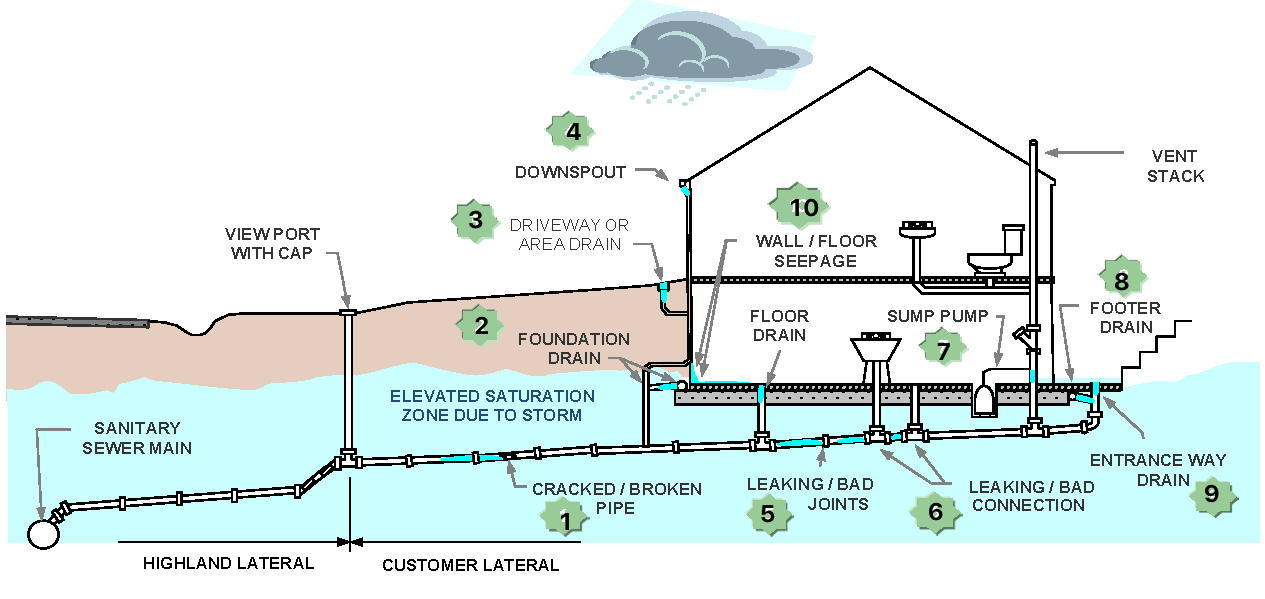
\includegraphics[width=6in]{InflowInfilatration1.jpg}
   \caption{Schematic of Inflow and Infiltration Sources}
   \label{fig:InflowInfilatration1} 
\end{figure}

\begin{table}[h!]
   \centering
   \caption{Inflow and Infiltration Source Classification}
   \begin{tabular}{c l  c} % Column formatting, @{} suppresses leading/trailing space
   ~ & ~ & \\
   \hline
   \hline
      Source ID & Source Name & Source Type (Inflow or Infiltration?) \\
      \hline
      1 &  Cracked/Broken Pipe &  \\
      2 &  Foundation Drain &  \\
      3 & Driveway or Area Drain &  \\  
      4 & Downspout   \\   
      5 & Leaking/Bad Joints &  \\ 
      6 & Leaking/Bad Connection &  \\
      7 & Sump Pump &  \\  
      8 & Footer Drain &  \\   
      9 & Entrance Way Drain & \\ 
      10 & Wall/Floor Seepage &  \\  
      \hline
      \hline
   \end{tabular}
   \label{tab:IandITwo}
\end{table}

\clearpage

\item (30 points) Figure \ref{fig:grainSize} is a grain size distribution curve for a soil sample in a receiving stream.
Figure \ref{fig:Hjulstrom} is a Hjulstrom diagram; 
\begin{figure}[ht!] %  figure placement: here, top, bottom, or page
\centering
   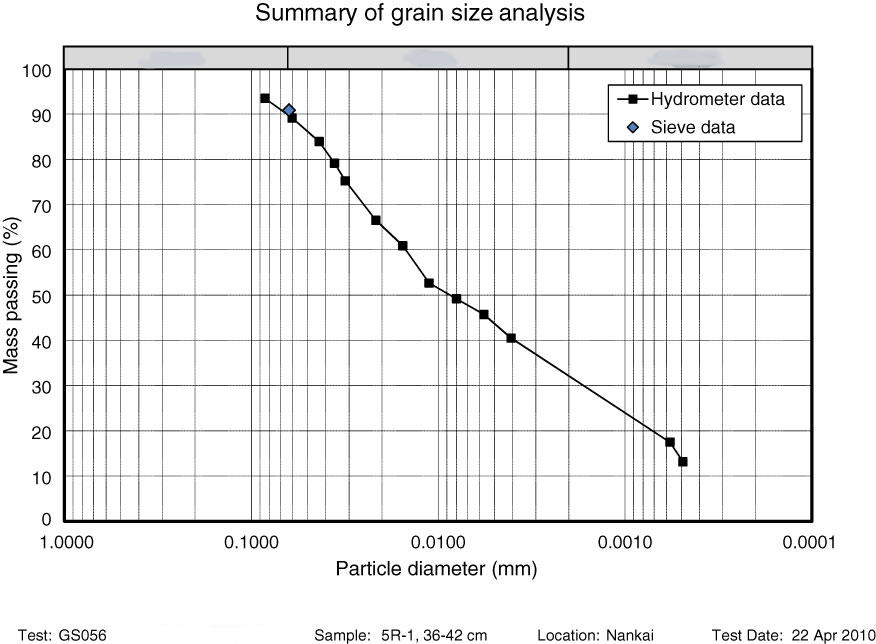
\includegraphics[height=3.4in]{grainSize.jpg}
   \caption{Grain Size Distribution for Nankai Outfall}
   \label{fig:grainSize} 
\end{figure}

\begin{figure}[ht!] %  figure placement: here, top, bottom, or page
\centering
   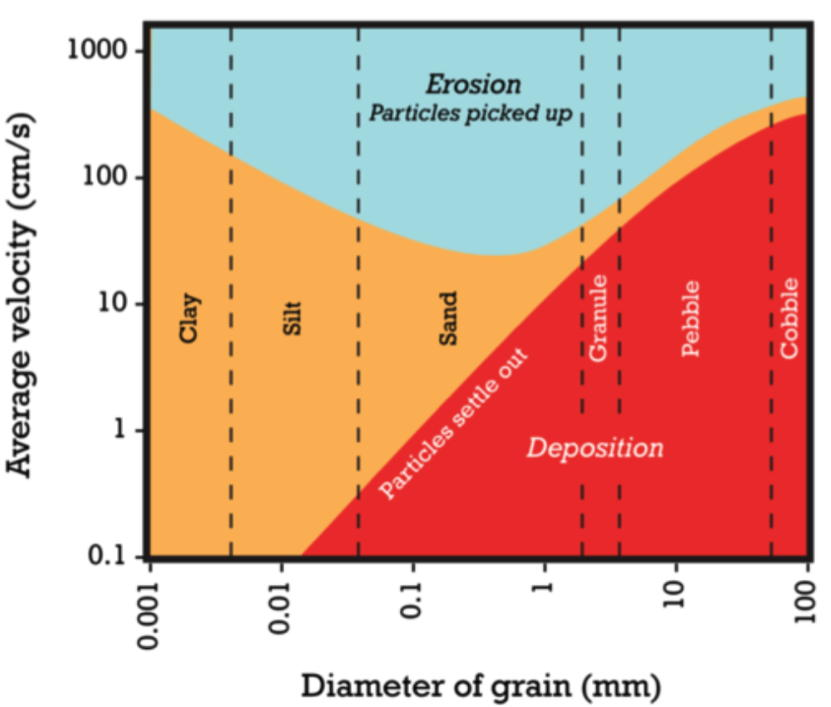
\includegraphics[height=3.4in]{Hjulstrom2.jpg}
   \caption{Hjulstrom Diagram for Sediment Transport}
   \label{fig:Hjulstrom} 
\end{figure}

\clearpage
Using the grain size distribution and the Hjulstrom diagram;

\begin{enumerate}[A)]
\item Estimate the median grain diameter, in millimeters.  Draw directly on the diagram to show where the mean grain size is plotted. ~\\
\item Estimate the \textbf{largest} particle diameter represented in the soil sample.  Draw directly on the diagram to show where the largest grain size is plotted. ~\\
\item Estimate the \textbf{smallest} particle diameter represented in the soil sample.  Draw directly on the diagram to show where the smallest grain size is plotted.
\item Draw directly on the diagram the three sizes determined above (smallest, median, and largest). ~\\ 
\item Determine the maximum stream velocity, in feet per second, at the outfall to prevent erosion if the smallest size is considered.
\item Determine the maximum stream velocity, in feet per second, at the outfall to prevent erosion if the median size is considered. 
\item Determine the maximum stream velocity, in feet per second, at the outfall to prevent erosion if the largest size is considered. ~\\
\item Determine the maximum stream velocity, in feet per second,  at the outfall to prevent erosion if no material in the sample is to be mobilized. ~\\
\end{enumerate}

\clearpage
%%%%%%%%%%%%%%%%%PROBLEM 2 LAZYBROOK %%%%%%%%%%%%%%%%%%
\item \label{prob:DrainDesign1} (100 points) Consider the drainage area depicted in Figure \ref{fig:Lazybrook}. 

\begin{figure}[ht!] %  figure placement: here, top, bottom, or page
\centering
   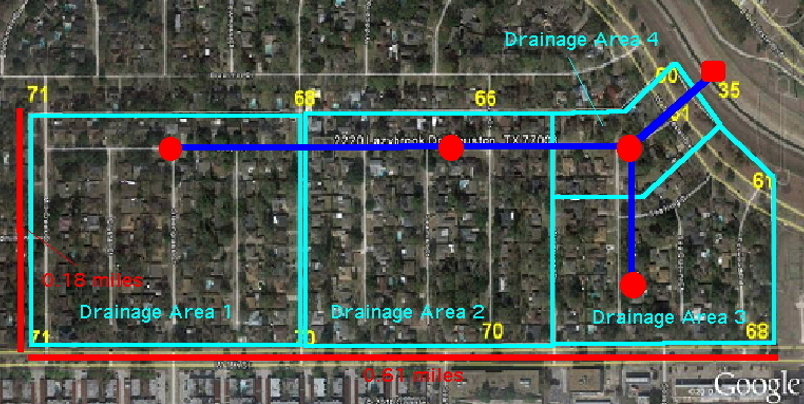
\includegraphics[width=6in]{lazybrook_drainage.png}
   \caption{Drainage System Layout}
   \label{fig:Lazybrook} 
\end{figure}

Table \ref{tab:drainageareas} lists the hydrologic features of the four drainage areas.
 
\begin{table}[ht!]
   %\centering
      \caption{Hydrologic data for each drainage area in Figure \ref{fig:Lazybrook} \\}
   %\topcaption{Table captions are better up top} % requires the topcapt package
   \begin{tabular}{| p{0.6in} | p{0.9in} | p{0.9in} | p{1.3in} | p{1.3in} |} % Column formatting, @{} suppresses leading/trailing space
   \hline
   \hline
Area ID & Area ($acres$) & Width ($feet$) & Avg. Slope ($\%$) & NRCS CN \\
\hline
\hline
DA\_1 &  25 & 1073 & 0.2 & 85\\
DA\_2 &  25 & 1073 & 0.2 & 85\\
DA\_3 &  17 & ~719 & 0.8 & 85\\
DA\_4 &  ~8 & ~688 & 0.9 & 85\\
\hline
\hline
   \end{tabular}
   \label{tab:drainageareas}
\end{table}



\begin{table}[ht!]
   %\centering
      \caption{Elevation data for each junction in Figure \ref{fig:Lazybrook} \\}
   %\topcaption{Table captions are better up top} % requires the topcapt package
   \begin{tabular}{| p{1.6in} | p{1.6in} | p{1.6in} |} % Column formatting, @{} suppresses leading/trailing space
   \hline
   \hline
Junction ID & Invert Elevation ($feet$) & Land Elevation ($feet$) \\
\hline
\hline
J-DA\_1 &  65 & 70 \\
J-DA\_2 &  60 & 66 \\
J-DA\_3 &  56 & 66 \\
J-DA\_4 &  48 & 62 \\
OUTFALL &  35 & N/A \\
\hline
\hline
   \end{tabular}
   \label{tab:junctions}
\end{table}

\clearpage
The red dots on Figure \ref{fig:Lazybrook} are inlets to the storm sewer system (indicated by the blue pipes).  The red rectangle (on the East side of the figure) is a stormwater outfall.  Table \ref{tab:junctions} lists the invert elevations, and land surface elevations of these points. 

The system is to be sized using the design storm shown in Table \ref{tab:storm}\footnote{A 10-inch, 24 hour, SCS Type-2 - with the first and last hour trimmed}

\begin{table}[ht!]
   %\centering
      \caption{Design Storm for Drainage System in Figure \ref{fig:Lazybrook} \\}
   %\topcaption{Table captions are better up top} % requires the topcapt package
   \begin{tabular}{| p{1.6in} | p{1.7in} |} % Column formatting, @{} suppresses leading/trailing space
   \hline
   \hline
Elapsed Time & Rainfall Intensity ($\frac{in}{hr}$) \\
\hline
\hline
00:00 & 0.11 \\
01:00 & 0.11 \\
02:00 & 0.13 \\
03:00 & 0.13 \\
04:00 & 0.15 \\
05:00 & 0.17 \\
06:00 & 0.19 \\
07:00 & 0.21 \\
08:00 & 0.27 \\
09:00 & 0.34 \\
10:00 & 0.54 \\
11:00 & 4.28 \\
12:00 & 1.09 \\
13:00 & 0.48 \\
14:00 & 0.34 \\
15:00 & 0.26 \\
16:00 & 0.22 \\
17:00 & 0.19 \\
18:00 & 0.17 \\
19:00 & 0.14 \\
20:00 & 0.13 \\
21:00 & 0.12 \\
22:00 & 0.12 \\
23:00 & 0.11 \\
\hline
\hline
   \end{tabular}
   \label{tab:storm}
\end{table}

The blue line segments on Figure \ref{fig:Lazybrook} are pipes that comprise the storm sewer system.   Table \ref{tab:pipes} lists the proposed design (i.e. pipe lengths, diameters, connection(s), and offsets) for the storm sewer.

\clearpage

\begin{table}[ht!]
   %\centering
      \caption{Hydraulic data for each pipe in Figure \ref{fig:Lazybrook} \\}
   %\topcaption{Table captions are better up top} % requires the topcapt package
   \begin{tabular}{| p{0.6in} | p{1.7in} | p{0.9in} | p{0.9in} | p{1.4in} |} % Column formatting, @{} suppresses leading/trailing space
   \hline
   \hline
Pipe ID & Connection (Start:End) & Diameter ($feet$) & Length ($feet$) & Offset (inlet:outlet) \\
\hline
\hline
P\_1 & DA\_1 : DA\_2 & 3.0 & 1000 & 0:0 \\
P\_2 & DA\_2 : DA\_4 & 3.0 & 1000 & 0:2 \\
P\_3 & DA\_3 : DA\_4 & 3.0 & 1000 & 0:2 \\
P\_4 & DA\_4 : OUTFALL & 5.0 & 1000 & 0:0\\
\hline
\hline
   \end{tabular}
   \label{tab:pipes}
\end{table}

Using these data build a SWMM model of the system.  Assume the outfall is a fixed pool with depth 5 feet (water elevation 40 feet).   Use DYNWAVE routing, and the SCS CN infiltration method in SWMM. 

Use the model to inform answers to:

\begin{enumerate}[A)]
\item Make a screen capture of your working model. ~\\~\\
\item How many subcatchments are in your model? ~\\~\\
\item Are all the pipes below grade?  ~\\~\\
\item Does the system surcharge during the design storm?  ~\\~\\
\item If yes, when does the surcharge occur (what time)? ~\\~\\
\item What is the maximum flow velocity in the sewer system?  ~\\~\\
\item Where does this maximum occur (which pipe)?  ~\\~\\
\item When does this maximum occur?  ~\\~\\
\item Use SWMM to sketch a profile of the sewer system and the water surface elevation at hour 12:00 of the simulation, starting at J-DA\_1 and ending at the OUTFALL ~\\~\\
\item Use SWMM to generate a time series (a plot) of the precipitation input  ~\\~\\
\item Use SWMM to generate a time series (a plot) of runoff in subcatchment DA\_2  ~\\~\\ 
\item Modify your model to make pipes P\_1 and P\_2, into 5.0 foot diameter pipes, keeping them at least 2 feet below grade.  ~\\~\\
\item List the required changes (there are several, invert elevations must be changed, and offsets need changing)
\item Does the system surcharge during the design storm?  ~\\~\\
\item Use SWMM to sketch a profile of the sewer system and the water surface elevation at hour 12:00 of the simulation, starting at J-DA\_1 and ending at the OUTFALL ~\\~\\
\item Use SWMM to generate a time series (a plot) of runoff in subcatchment DA\_2  ~\\~\\
\end{enumerate}
\clearpage



\end{enumerate}



\end{document}  
